\scanpage{37}
% archive sheet number: 36
$K\subset\mathbb C$, $\bar K$ clôture alg. dans $\mathbb C$, $\pi_1=\pi_1(\mathrm{Spec}\,K,\bar K)=\mathrm{Gal}(\bar K/K)$, $\unsure{A|\mathcal A}={}$anneau des adèles ``finis'' de $\mathbb Q$. On \unsure{$^{1}$|$^{l}$}considère une catégorie de motifs sur $K$, de type fini, et le groupe de Galois \inserted{$G$} associé au foncteur de Betti. Cela donne naissance aux structures suivantes.

% Diagram across the head of the sheet; the small boxes share their frames' corners.
\diagram{\resizebox{\linewidth}{!}{\begin{tikzcd}[ampersand replacement=\&,column sep=4pt,row sep=7pt,execute at end picture={
 \draw ([xshift=-5pt,yshift=6pt]gd.north west) rectangle ([xshift=5pt,yshift=-8pt]gp.east |- gm.south);
 \node[draw,anchor=south east,inner sep=1pt] at ([xshift=5pt,yshift=-8pt]gp.east |- gm.south) {$D$};
 \draw ([xshift=-5pt,yshift=6pt]p.north west) rectangle ([xshift=5pt,yshift=-12pt]g.south east);
 \node[draw,anchor=south east,inner sep=1pt] at ([xshift=5pt,yshift=-12pt]g.south east) {$B$};
 \draw (p.south) -- (avec.north);
 \draw (conn.center) ellipse [x radius=38pt,y radius=13pt];
 \draw (pc.south) -- (ptc.north);
 \draw (qc.south) -- (ptq.north);
 \draw (ptc.center) ellipse [x radius=37pt,y radius=14pt];
 \node[draw,anchor=south east,inner sep=1pt] at ([xshift=5pt,yshift=-3pt]ptc.south east) {$C$};
 \node[draw,anchor=south east,inner sep=1pt] at (ga.south east) {$A$};
}]
 |[alias=gd]| G''_K \arrow[r,phantom,"{\supset}" description] \& H''_K\arrow[r,dash,dashed] \& Q\arrow[r,dash,dashed] \& H'_K \&[-4pt] {\subset} \&[-4pt] |[alias=gp]| G'_K\arrow[r,dash,dashed] \& |[alias=p]| P\arrow[r,dash,dashed] \& |[alias=g]| G_K \&[13pt] |[alias=pc]| P_{\mathbb C} \& G_{\mathbb C} \& |[alias=qc]| Q_{\mathbb C} \&[8pt] |[draw,alias=ga,minimum width=34pt,minimum height=24pt]| G\\
 |[alias=gm]| \mathbb G_m\arrow[u,shift left=1,"i_1"]\arrow[u,shift right=1,"i_2"'] \& \& \& \& \& \& |[alias=avec]| \text{avec} \& \& |[alias=ptc]| \begin{gathered}\text{avec pt }\deleted{\unsure{\xi|a}}\ \alpha\\\text{rat}/\mathbb C,\ \text{de}\end{gathered} \& \& |[alias=ptq]| \begin{gathered}\text{avec pt }\unsure{\xi_1|\alpha_1}\\\text{rat}/\mathbb C,\end{gathered} \& \\
 \& \& \& \& \& \& |[alias=conn]| \begin{gathered}\text{connexion absolue}\\\text{intégrable}\end{gathered} \& \& \text{sorte que} \& \& \& \\
 \& \& \& \& \& \& \begin{gathered}\text{invariante}\\\text{par }G_K\\{}[\,\text{NB structure vide}\\\text{si }K\ \text{abst. alg}\,]\end{gathered} \& \& \& \& \&
\end{tikzcd}}}

\diagram{\begin{tikzcd}[ampersand replacement=\&,column sep=25pt,execute at end picture={\draw ([xshift=-3pt,yshift=6pt]pu.north west) rectangle ([xshift=4pt,yshift=-4pt]gu.south east); \node[draw,anchor=south east,inner sep=1pt] at ([xshift=4pt,yshift=-4pt]gu.south east) {$G$};}]
 |[alias=pu]| \pi_1 \arrow[r,"{\substack{\deleted{\unsure{v|w}}\\u}}"] \& |[alias=gu]| G(A)
\end{tikzcd}}
\[
 \deleted{(\pi_1)_{\mathbb Q}\xrightarrow{\unsure{v|u}}G/G^\circ\quad\text{i.e.}\quad\pi_1\to(G/G^\circ)(\mathbb Q)}
\]

\uline{NB} La donnée \deleted{\unsure{principale}} compliquée $\boxed D$ peut être remplacée par la ``donnée subordonnée'' $\boxed E$, \uline{soumise} à la condition d'être ``compatible'' avec $A,B,C$

a) la connexion absolue définit
\[
 \omega\in\Omega^1_{\mathbb C/\mathbb Q}\otimes_{\mathbb Q}{\mathfrak g}_{\mathbb Q}
\]

b)
\diagram{\begin{tikzcd}[ampersand replacement=\&,column sep=0pt,row sep=0pt]
 G' \& \otimes_K\mathbb C \&[5pt] \simeq \&[5pt] G_{\mathbb C}\\
 {\rotatebox{90}{$\subset$}} \& \& \&\\
 H' \& \otimes_K\mathbb C \& \&\\
 {\rotatebox{90}{$\simeq$}} \& \& \&\\
 H'' \& \otimes_K\mathbb C \& \&\\
 {\rotatebox{90}{$\simeq$}} \& \& \&\\
 G''_1 \& \otimes_K\mathbb C \& \simeq \& G_{\mathbb C}
\end{tikzcd}}

c) d'où des hom
\diagram{\begin{tikzcd}[ampersand replacement=\&,row sep=1pt,column sep=8pt]
 \& \& \boxed E\arrow[d]\\
 i_1^{\mathbb C},\nu_2^{\mathbb C}:G_{m\,\mathbb C}\arrow[r] \& G_{\mathbb C} \& {}
\end{tikzcd}}

d) On a, pour un modèle régulier convenable $S$ de $K$, de type fini sur $\mathbb Z$ (supposons $K$ de t.f. sur $\mathbb Q$)
\diagram{\begin{tikzcd}[ampersand replacement=\&,column sep=16pt,row sep=5pt,execute at end picture={\draw ([xshift=-4pt]ds.south east) |- ([xshift=2pt,yshift=2pt]geom.north);}]
 \& \& \boxed G\\
 |[alias=ds]| \pi_1(S(\mathbb C),{\unsure{\xi|\zeta}})\arrow[r,"w"] \& G(\mathbb C). \&\\
 |[alias=geom]| \begin{gathered}\text{pt géom}\\\text{déduit de}\\\text{l'inclusion}\\K\subset\mathbb C\end{gathered} \& \begin{gathered}{}[\,\text{NB : structure}\\\text{vide si }K\text{ est}\\\text{abst. alg.}\,]\end{gathered}\&
\end{tikzcd}}

% The line running from e) meets the lower right corner of the boxed consequence.
\diagram{\resizebox{\linewidth}{!}{\begin{tikzcd}[ampersand replacement=\&,column sep=9pt,row sep=5pt,execute at end picture={
 \coordinate (cl) at ([xshift=-4pt]lh.west);
 \coordinate (cr) at ([xshift=6pt]qr.east);
 \draw ([yshift=3pt]cl |- lh.north) rectangle ([yshift=-4pt]cr |- lb.south);
 \draw ([xshift=-13pt,yshift=-9pt]lh.west) circle [radius=2pt];
 \draw ([xshift=-13pt,yshift=-9pt]lh.west) -- ([xshift=1pt,yshift=5pt]lh.north west);
 \draw[rounded corners=6pt] ([xshift=-8pt,yshift=1pt]eb.south west) -- ([xshift=-4pt,yshift=-4pt]cr |- lb.south) -- ([xshift=-6pt,yshift=6pt]et.north west) -- ([xshift=8pt,yshift=4pt]et.north east) -- ([xshift=10pt,yshift=-1pt]eb.south east) -- ([xshift=-8pt,yshift=-2pt]eb.south west) -- cycle;
}]
 |[alias=lh]| \text{Il en résulte aussi que le diagramme} \& {} \&[25pt] {}\\
 \pi_1(S(\mathbb C),\xi)\arrow[r,"{\unsure{w|{}}}"]\arrow[d,"\mathrm{can.}"] \& |[alias=qr]| G(\mathbb Q)\arrow[d] \& |[alias=et]| \begin{gathered}\text{e) }P/G^\circ\text{ est un}\\\text{torseur sur }K,\ \text{de}\end{gathered}\\
 \pi_1(S,\xi)\arrow[r,"v"] \& G/G^\circ(\mathbb Q) \& \begin{gathered}\text{groupe }G/G^\circ,\ \text{ponctué}\\\text{par }\xi:K\to\mathbb C,\ \text{donc}\end{gathered}\\
 |[alias=lb]| \text{est commutatif} \& {} \& |[alias=eb]| \begin{gathered}\text{définit}\quad v:\pi_1\longrightarrow(G/G^\circ)(\mathbb Q)\\\text{i.e.}\quad\pi_1\longrightarrow(G/G^\circ)_{\mathbb Q}\end{gathered}
\end{tikzcd}}}

\uline{Propriétés}

1) $i_2^{\mathbb C}=\overline{i_1^{\mathbb C}}$ (donc $\unsure{\alpha_1|\alpha}$ est connu quand on connaît $\alpha$)

2) $\pi_1(S(\mathbb C),\xi)\to G(\mathbb C)$ se factorise par $G(\mathbb Q)$, \deleted{et on a \unsure{compatibilité}}

3) $\pi_1\to G(A)$ se factorise par $\pi_1(S,\xi)\unsure{\mathrel{-}|\to}G(A)$ pour $S$ convenable

4) les diagr.
\diagram{\begin{tikzcd}[ampersand replacement=\&,column sep=27pt]
 \pi_1(\deleted{\unsure{S|C}}S(\mathbb C)\deleted{\unsure{,\xi|)}} ,\xi)\arrow[r,"{\deleted{\unsure{\pi_1|u}}}","w"']\arrow[d,"\mathrm{can.}"] \& G(\mathbb Q)\arrow[d,"\mathrm{can.}"]\\
 \pi_1(S,\xi)\arrow[r,"u"] \& G(A)
\end{tikzcd}\hspace{5pt}\begin{tikzcd}[ampersand replacement=\&,column sep=13pt]
 \pi_1\arrow[r,"v"]\arrow[d,"u"] \& G/\deleted{\unsure{G'|G}}G^\circ(\mathbb Q)\arrow[d]\\
 \deleted{\unsure{u|G}}G(A)\arrow[r] \& (G/G^\circ)(A)
\end{tikzcd}}
\unsure{sont|\deleted{sont}} commutatifs. \unsure{!|/}

5) Le composé $\pi_1(S,\xi)\mathrel{-}G(A)\xrightarrow{\varepsilon}A^*$ est l'hom défini par l'action de $\pi_1(S,\xi)$ sur les racines de l'unité.

% This addition occupies the lower right of the sheet. Its linking stroke begins after 5).
\figure{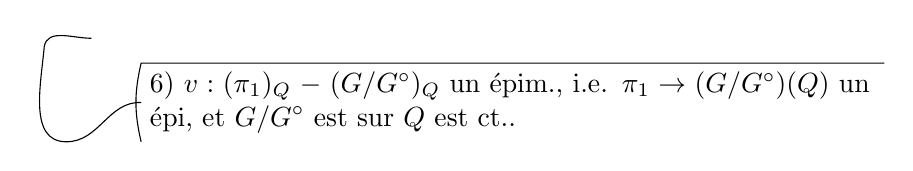
\begin{tikzpicture}
 \node[inner sep=3pt,text width=.76\linewidth,align=left] (addsix)
 {\inserted{6) $v:(\pi_1)_{\mathbb Q}\mathrel{-}(G/G^\circ)_{\mathbb Q}$ un épim., i.e. $\pi_1\to(G/G^\circ)(\mathbb Q)$ un épi, et $G/G^\circ$ \deleted{\unsure{est}} sur $\mathbb Q$ est \uuline{ct.}.}};
 \draw (addsix.north east) -- (addsix.north west) to[bend right=13] (addsix.south west);
 \draw (addsix.west) to[out=178,in=0] ([xshift=-27pt]addsix.south west) to[out=180,in=-95] ([xshift=-35pt,yshift=6pt]addsix.north west) to[out=80,in=180] ([xshift=-18pt,yshift=9pt]addsix.north west);
\end{tikzpicture}}

\deleted{\unsure{6|7}}7) Pour tout point fermé $s$ de $S$, l'élément de \unsure{frobénius|frobènius} $f_s$ de $\pi_1(S,\xi)$ a \deleted{comme image} \inserted{une} classe dans $G(A)$ \inserted{qui correspond à} l'image d'une classe de conjugaison de $G\deleted{\unsure{(A)|_{\mathbb Q}}}$ (redonne Weil \unsure{...|....}).

% slanted
\margin{devra être \unsure{précisé|precisé} ...}

\deleted{\unsure{7|8}}8) $G_{\mathbb R}$ muni de $i_1^{\mathbb C},i_2^{\mathbb C}$ de c) est un \uline{groupe de Hodge}.

\deleted{\unsure{8|9}}9) (Modulo Tate) Pour tout $\unsure{l|\ell}$, l'image de $\pi_1\unsure{k|K|\xi}$ dans $G(\mathbb Q_l)$ est un sous-groupe opérant de façon $\frac12$ simple sur tout \deleted{\unsure{produit|foncteur|générateur}} $V\otimes_{\mathbb Q}\mathbb Q_l$ \deleted{\unsure{engendre|engendré} $\mathbb Q_l$ comme}, (ou \uline{un} tel, avec $\deleted{\unsure{V|D}}V$ \deleted{seul} fidèle), et son enveloppe algébrique est $G_{\mathbb Q_l}$.

\deleted{\unsure{Le composé} $\pi_1\to G(A)\to G(\mathbb Q_l)\unsure{\mathrel{-}|\to}G/G^\circ$}

% paper watermark, sideways
{\centering \textsc{\unsure{Extra} \unsure{Strong}}\\
\textit{\unsure{Ma}\unsure{in|nn}\unsure{ol|on}\unsure{uy|ny|y} \unsure{1808}}\par}
